\documentclass{article}
\usepackage[utf8]{inputenc}
\usepackage{gensymb}
\usepackage{graphicx}
\usepackage{parskip}
\usepackage{datetime}
\usepackage{amsmath, bm}

\newcommand{\HRule}{\rule{\linewidth}{0.5mm}}

\newdateformat{monthyear}{\monthname[\THEMONTH], \THEYEAR}

\begin{document}

\pagenumbering{gobble}

\begin{center}

\HRule \\[0.4cm]
{ \huge \bfseries Lab 2: INS and Kalman Filter \\[0.4cm] 
\Large \bfseries TTK5: Kalman Filtering and Navigation \\[0.4cm] } 

\HRule \\[1.5cm]

\begin{center} \large
\emph{By:}\\
\textbf{Andreas Nordby Vibeto}\\
andvibeto@gmail.com \\
(andreanv@stud.ntnu.no)
\end{center}

\vfill

{\large \monthyear\today}

\end{center}
\newpage
\pagenumbering{arabic}

\section*{Task 1}
\begin{figure}[!ht]
    \centering
    \makebox[\textwidth][c]{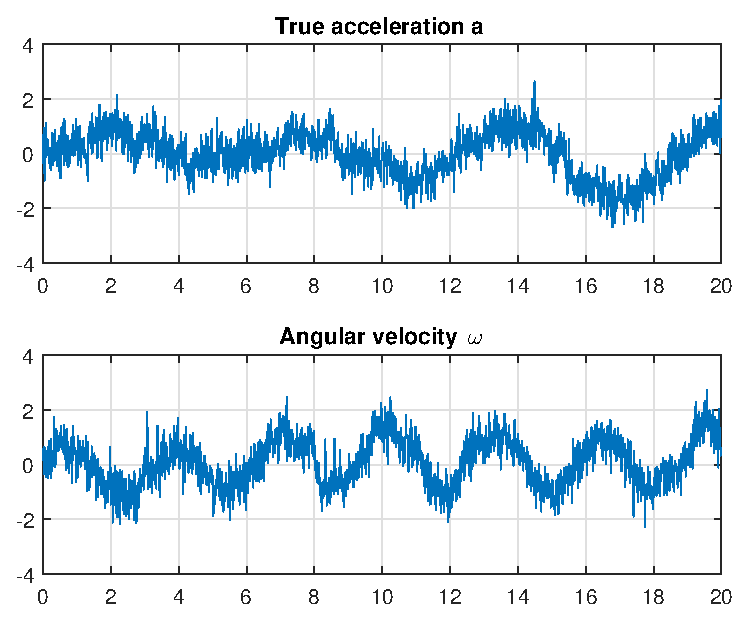
\includegraphics[width=1.25\textwidth, keepaspectratio=true]{../src/task1.eps}}
    \caption{True acceleration and angular velocity.}
\end{figure}

\section*{Task 2}
In order to discretize the system, it must first be written as a state space model. The system

\begin{subequations}
\begin{equation}
	\dot{x} = v 
\end{equation}
\begin{equation}
	\dot{v} = a
\end{equation}
\begin{equation}
	\dot{\theta} = \omega
\end{equation}
\end{subequations}

can be written as

\begin{subequations}
\begin{equation}
	\dot{\bm{x}} = \bm{A}\bm{x} + \bm{B}\bm{u}
\end{equation}
\begin{equation}
	\begin{bmatrix}
		\dot{x} \\ \dot{v} \\ \dot{\theta}
	\end{bmatrix}
	=
	\begin{bmatrix}
		0 & 1 & 0 \\
		0 & 0 & 0 \\
		0 & 0 & 0
	\end{bmatrix}
	\begin{bmatrix}
		x \\ v \\ \theta
	\end{bmatrix}
	+
	\begin{bmatrix}
		0 & 0 \\
		1 & 0 \\
		0 & 1
	\end{bmatrix}
	\begin{bmatrix}
		a \\ \omega
	\end{bmatrix}
	.
\end{equation}
\end{subequations}

By using forward Euler to discretize the system, it can be written on the form

\begin{equation}
	\label{eq:euler}
	\bm{x}(t_{k+1}) = (\bm{I} + h\bm{A}(t_k))\bm{x}(t_k) + h\bm{B}(t_k)\bm{u}(t_k)
\end{equation}

where $h$ is the step size. The discretized system then becomes

\begin{equation}
	\bm{x}(t_{k+1}) =
	\begin{bmatrix}
		1 & h & 0 \\
		0 & 1 & 0 \\
		0 & 0 & 1
	\end{bmatrix}
	\bm{x}(t_k) + 
	\begin{bmatrix}
		0 & 0 \\
		h & 0 \\
		0 & h
	\end{bmatrix}
	\bm{u}(t_k).
\end{equation}

Figure \ref{fig:disc_states} shows plots of the states in the discretized system.

\begin{figure}[!ht]
    \centering
    \makebox[\textwidth][c]{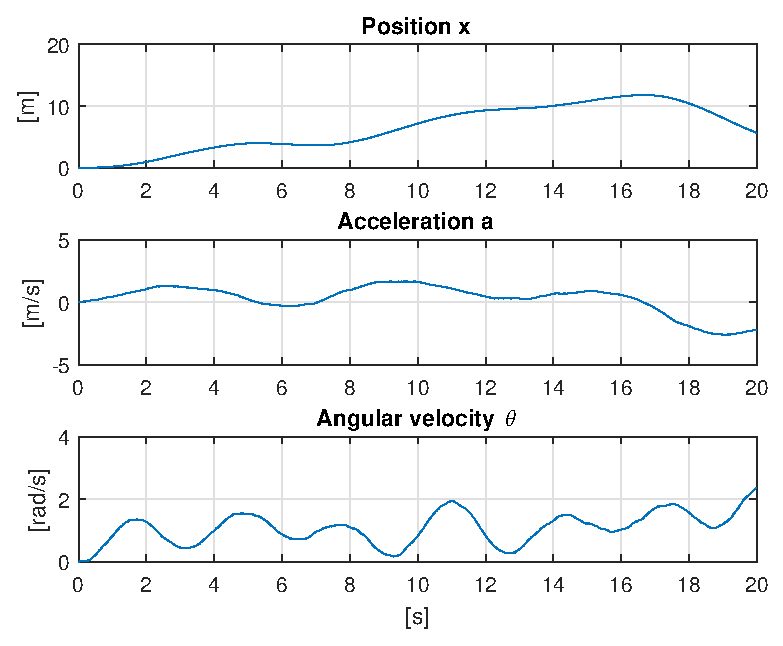
\includegraphics[width=1.25\textwidth, keepaspectratio=true]{../src/disc_states.eps}}
    \caption{States of the discretized system.}
    \label{fig:disc_states}
\end{figure}


\section*{Task 3}
When white noise is expressed in discrete time it is referred to as a white sequence \cite{heftet}, where the sequence consists of random variables that are uncorrelated \cite{wikiWhite}. The autocorrelation function for discrete white noise is:

\begin{equation}
	R_d(k) = A\delta(k) , \hspace{5pt} \delta(k) =
	\begin{cases}
		1 \hspace{10pt} k = 0 \\
		0 \hspace{10pt} k \neq 0
	\end{cases}.
\end{equation}

When using Matlab, white Gaussian noise can be generated by using \texttt{wgn()}, which will generate a sequence of uncorrelated random variables, which can be regarded as a white sequence.

The biases $b_1$ and $b_2$ can be discretized with forward Euler using equation \ref{eq:euler} from task 2. The bias can be written in state space form as

\begin{equation}
	\dot{\bm{x}} = 
	\begin{bmatrix}
		-\frac{1}{T_1} & 0 \\
		0 & -\frac{1}{T_2}
	\end{bmatrix}
	\bm{x} +
	\begin{bmatrix}
		1 & 0 \\
		0 & 1
	\end{bmatrix}
	\bm{w}
\end{equation}

where

\begin{center}
\begin{math}
	\bm{x} =
	\begin{bmatrix}
		b_1 \\ b_2
	\end{bmatrix}
	, \hspace{5pt} \bm{w} =
	\begin{bmatrix}
		w_1 \\ w_2
	\end{bmatrix}
	.
\end{math}
\end{center}

The resulting discretized system is:

\begin{equation}
	\bm{x}(t_{k+1}) =
	\begin{bmatrix}
		1 - \frac{h}{T_1} & 0 \\
		0 & 1 - \frac{h}{T_2}
	\end{bmatrix}
	\bm{x}(t_k) +
	\begin{bmatrix}
		h & 0 \\
		0 & h
	\end{bmatrix}
	\bm{w}(t_k).
\end{equation}



\newpage
\addcontentsline{toc}{chapter}{References}
\begin{thebibliography}{25}

	\bibitem{heftet}
	Vik, Bjørnar (2014)
	\emph{"Integrated Satellite and Inertial Navigation Systems"},
	Norwegian University of Science and Technology, Department of Engineering Cybernetics, Trondheim
	
	\bibitem{wikiWhite}
	Wikipedia,
	\emph{https://en.wikipedia.org/wiki/White\_noise},
	accessed 05.11.2016
	
\end{thebibliography}

\end{document}